\documentclass[fleqn]{article}
\oddsidemargin 0.0in
\textwidth 6.0in
\thispagestyle{empty}
\usepackage{import}
\usepackage{amsmath}
\usepackage[backend=bibtex]{biblatex}
\usepackage[utf8]{inputenc}
\usepackage{csquotes}
\usepackage{graphicx}
\usepackage{flexisym}
\usepackage{calligra}
\usepackage{amssymb}
\usepackage{bigints} 
\usepackage[english]{babel}
\usepackage{float}
\usepackage[colorinlistoftodos]{todonotes}
\usepackage{blindtext}
\usepackage{hyperref}

\addbibresource{references.bib}

\hypersetup{
  colorlinks=true,
  linkcolor=blue,
  filecolor=magenta,      
  urlcolor=cyan,
  pdfpagemode=FullScreen
}

\DeclareMathAlphabet{\mathcalligra}{T1}{calligra}{m}{n}
\DeclareFontShape{T1}{calligra}{m}{n}{<->s*[2.2]callig15}{}
\newcommand{\scriptr}{\mathcalligra{r}\,}
\newcommand{\boldscriptr}{\pmb{\mathcalligra{r}}\,}


\setlength{\arrayrulewidth}{0.5mm}
\setlength{\tabcolsep}{18pt}
\renewcommand{\arraystretch}{1.5}

\definecolor{hwColor}{HTML}{AD53BA}

\begin{document}

  \begin{titlepage}

    \newcommand{\HRule}{\rule{\linewidth}{0.5mm}}

    \center

    \begin{center}
      
\includegraphics[height=11cm, width=11cm]{asu.png}
    \end{center}

    \vline

    \textsc{\LARGE Advanced Laboratory I}\\[1.5cm]

    \HRule \\[0.5cm]
    { \huge \bfseries Pulsed NMR}\\[0.4cm] 
    \HRule \\[1.0cm]

    \textbf{Behnam Amiri}

    \bigbreak

    \textbf{Prof: Ralph Chamberlin}

    \bigbreak

    \textbf{Lab Partners: Daniel Henningsen, Micah Smith, Srihari Ravi}

    \bigbreak

    \textbf{{\large \today}\\[2cm]}

    \vfill

  \end{titlepage}

  \textbf{Abstract}

  \vspace{10px}

  This lab report represents the experimental procedure we did to learn about the \emph{Photon Interference} which is to demonstrate 
  the wave-particle duality of light by "\emph{measuring the existence of interference}." \textcite{One}

  \vspace{20px}


  \textbf{I. Introduction}

  \vspace{10px}


  \textbf{II. Background Information}

  \vspace{10px}


  \textbf{III. Theory}

  \vspace{10px}


  \textbf{IV. Experimental Procedure}

  \vspace{10px}

  We just followed the given steps in the lab. 
  

  \textbf{V. Results}

  \vspace{10px}

    
  \begin{figure}[h!]
    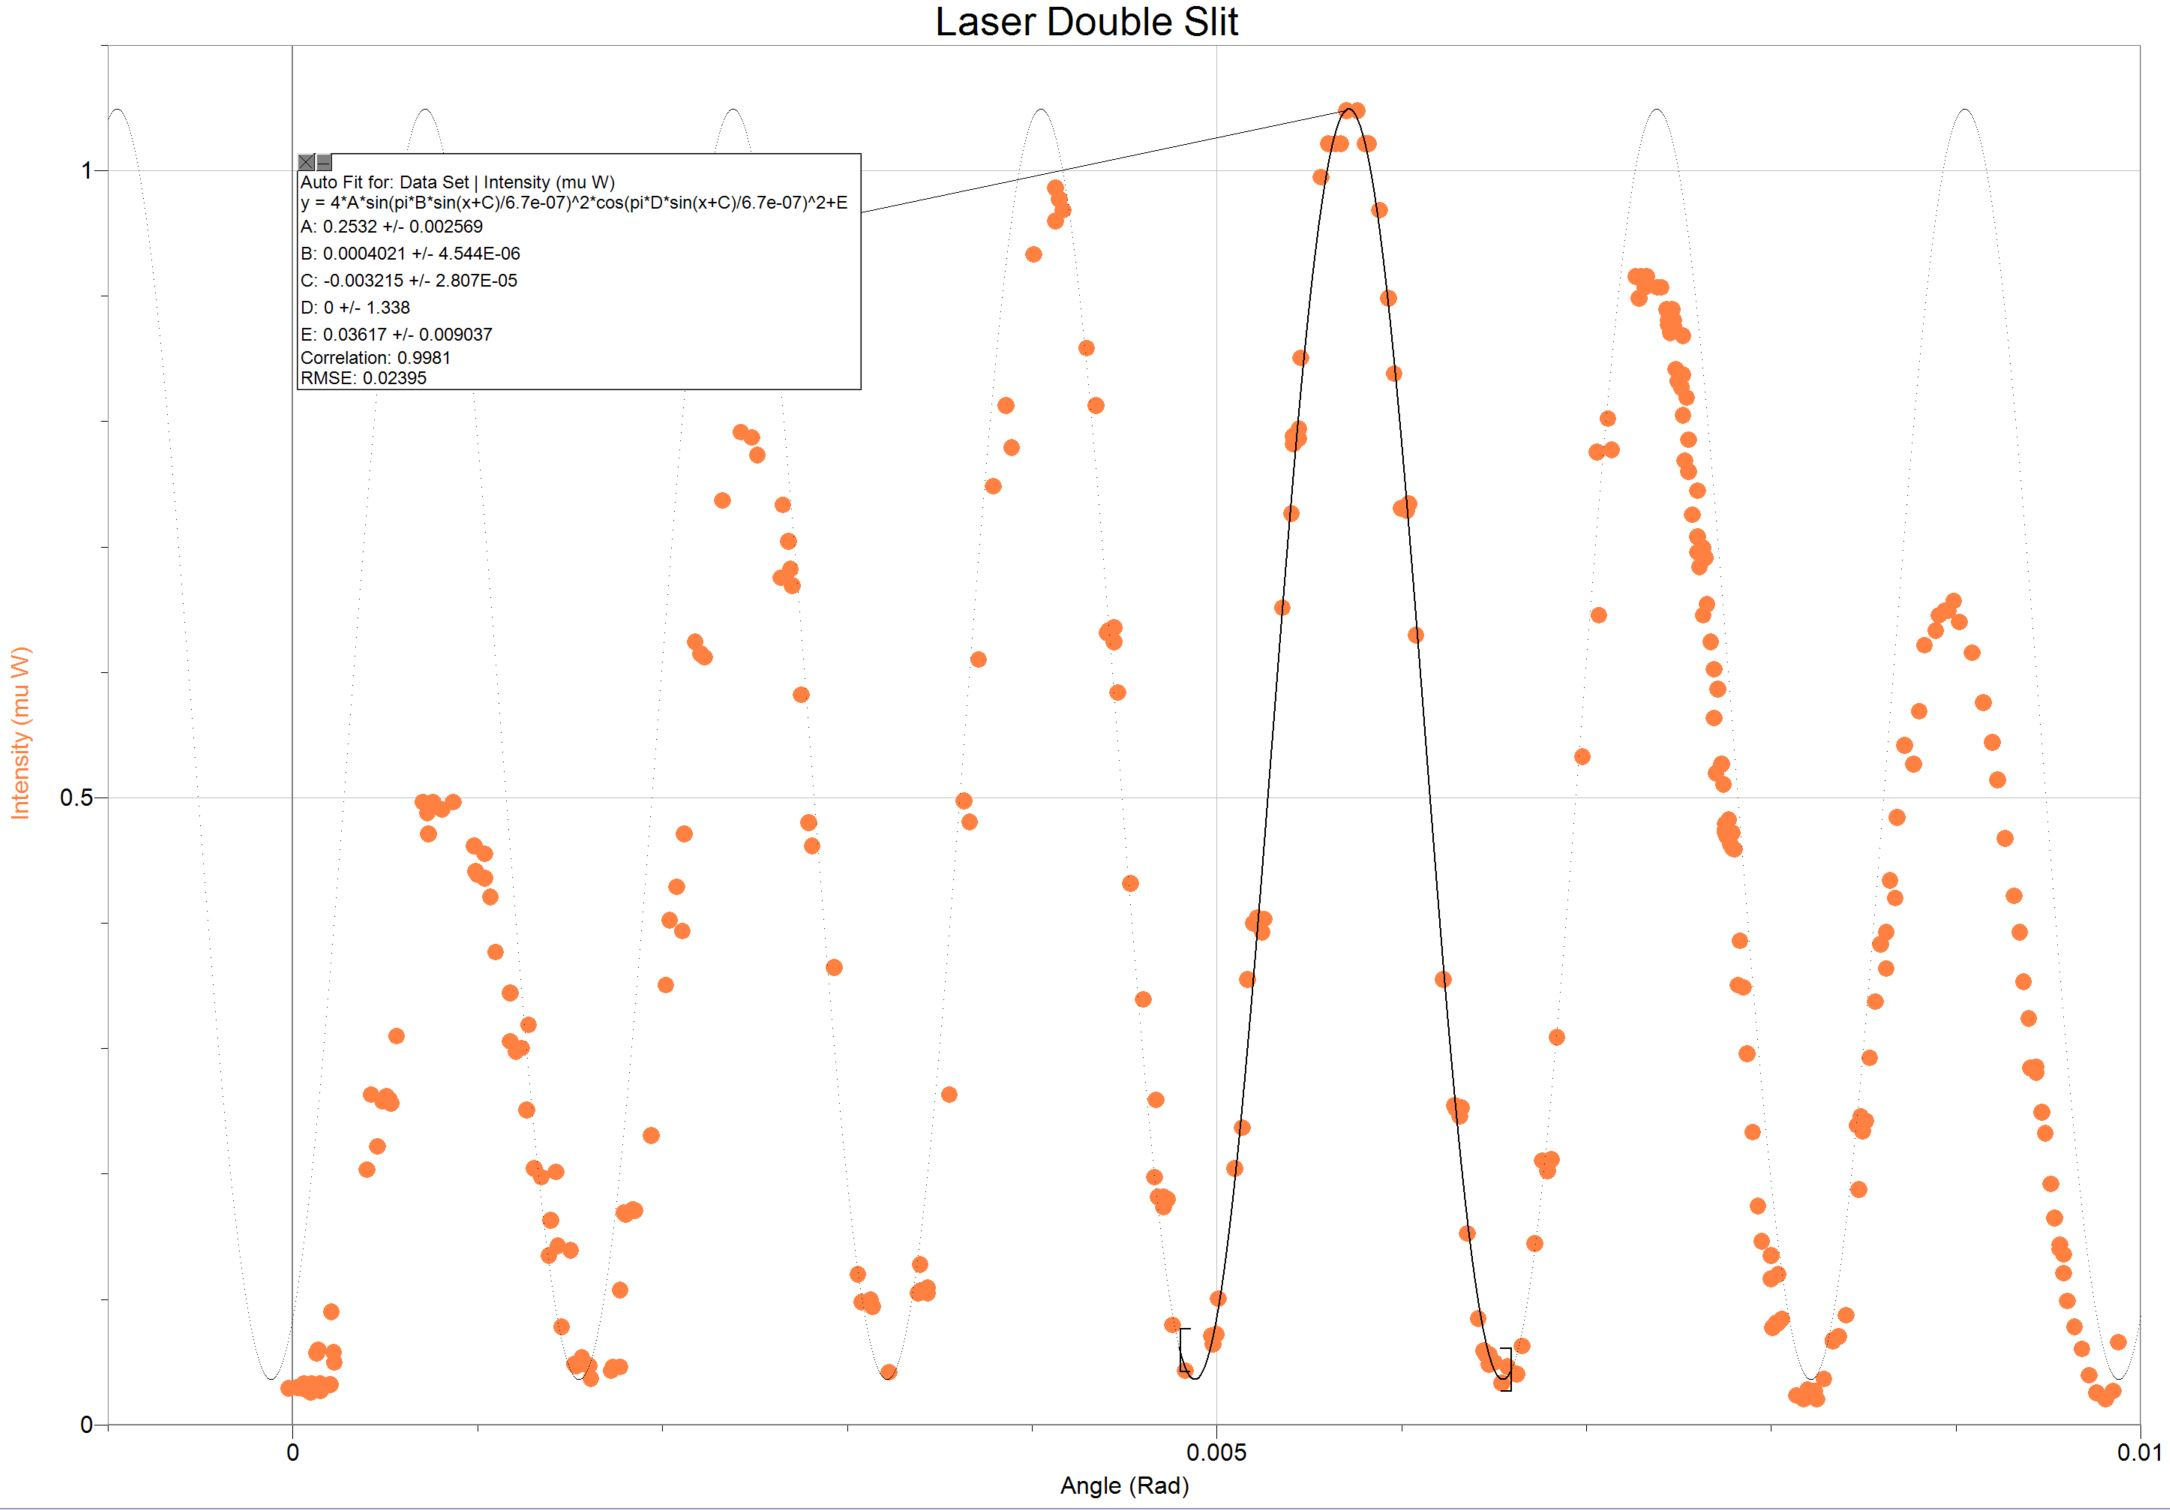
\includegraphics[height=12cm, width=18cm]{Fig1.JPG}
    \caption{
      Laser Double-Slit. rtion of the diffraction
      pattern.
    }
  \end{figure}

  \pagebreak

  \textbf{VI. Discussion}

  \vspace{10px}

  In this experiment 
  
  \vspace{20px}


  \textbf{VII. Conclusions}

  \vspace{10px}

  Light is very 
  
  \vspace{20px}


  \printbibliography

\end{document}
